\documentclass{article}
\usepackage[russian]{babel}
\usepackage[utf8]{inputenc}
\usepackage{lpic}
\usepackage[usenames,dvipsnames]{xcolor}
\usepackage{punk}
\usepackage[T1]{fontenc}
\pagestyle{empty}
\usepackage{tikz}
\usepackage[papersize={12.782in,9.250in}, spine=0.532in, cropgap=0.125in
%,cropmarks,cropframe
]{zwpagelayout}%0.125" + 6" + 192*0.002252" + 6" + .125" =  12.682384

%\usepackage{pstricks}
\usepackage{tikz}\usetikzlibrary{calc,shadows}

\usepackage[pages=some]{background}

\backgroundsetup{
scale=1,
opacity=1,
angle=0,
contents={%
  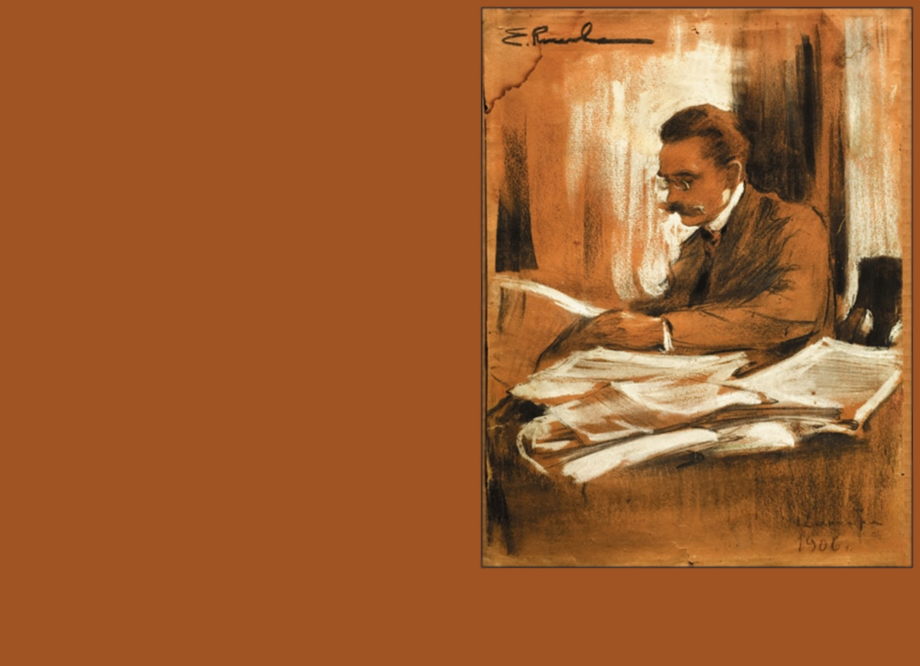
\includegraphics[scale=1]{kiselyov}
  }%
}

\makeatletter
\DeclareRobustCommand\vttfamily{%
  \not@math@alphabet\vttfamily\relax
  \fontfamily{cmvtt}% cmvtt (Computer Modern) or lmvtt (Latin Modern)
  \selectfont
}
\DeclareTextFontCommand{\textvtt}{\vttfamily}
\makeatother

\begin{document}

\BgThispage

\begin{tikzpicture}
[ overlay,
    remember picture,
    mynode/.style={left,fill=yellow!10,general shadow={shadow scale=1, shadow xshift=-0.8ex, shadow yshift=-0.8ex,
opacity=1, fill=gray!50}},
]

\node[below] at ($(current page.south east)+(-3in,1.2in)$) {
\ttfamily\bfseries\Huge{\color{yellow!10}  Геометрия по Киселёву}};
    \node[rotate=90] at ($.5*(current page.south east)+.5*(current page.north west)$) {
\ttfamily\bfseries\LARGE{\color{yellow!10}  ГЕОМЕТРИЯ ПО КИСЕЛЁВУ}};
    \node[above right, fill=yellow!10] at ($(current page.south west)+(3in,+.2in)$) {\includegraphics[scale=1]{isbn_barcode}};
    
  \node[below right] at ($(current page.north west)+(.5in,-.5in)$) {  \hbox{
\hspace{3em}\parbox{.35\textwidth}
{\vttfamily\large 
{\color{yellow!10}Новое издание классического школьного учебника по геометрии. За основу взято издание 1938 года, но использовались также издания 1914 и 1931 годов.}
}}};

\end{tikzpicture}

\end{document}

\psset{unit=1in}
\begin{pspicture}(12.782,9.250)% use your page size
  \rput[r](6,-4){\parbox{8in}{\begin{flushright}
    \ttfamily\bfseries\LARGE{\color{white}  Геометрия по Киселёву}
    \end{flushright}}}
  %\uput[-90](3.5,8){\color{red}\rule{5}{1ex}}
  % ...
\end{pspicture}

==============

\begin{lpic}[t(-1.05in),b(0mm),r(0mm),l(5.45in)]{isbn_barcode(1)}
\lbl[b]{120,-23;{\hbox{
\parbox{.5\textwidth}{\begin{center}
        \ttfamily\bfseries\Huge{\color{white}  Геометрия по Киселёву}                           
                                 \end{center}
}}}}
\lbl{120,-25;{\ttfamily\LARGE {\color{white}Планиметрия}}}
\lbl[]{-9,200,90;{\ttfamily\bfseries\LARGE  {\color{white}  ГЕОМЕТРИЯ ПО КИСЕЛЁВУ}}}
\end{lpic}
